\documentclass[a4paper,10pt]{article}
%\documentclass[a4paper,10pt]{scrartcl}
\usepackage{hyperref}
% \usepackage{caption}
\hypersetup{pdfborder={0 0 0}}
\usepackage[all]{hypcap}
\usepackage{default}
\usepackage{graphicx}
\usepackage{array}
\usepackage{amsmath}
\usepackage{listings}
\usepackage {apacite}
\lstset{language=Python,% general command to set parameter(s)
basicstyle =\small\ttfamily,          % print whole listing small
showstringspaces=false,
commentstyle=\ttfamily}

\title{Backpropagation in Feedforward Networks}
\author{Dr. Olivia Guest}
\date{\today}

\begin{document}
\maketitle
\section{Overview}
Last week we ran and trained a 2-layer perceptron. For reasons that became obvious (i.e., if no linear separation of the target states can be accomplished) 2-layer perceptrons are not as useful as one might initially assume. For this reason, we must turn to adding a 3rd layer of units between the input and the output units. This as you might expect is called the hidden layer because they are neither input nor output units --- their activations are not directly in contact with the environment the network is in. Adding hidden units produces a 3-layer perceptron. As we shall see it can now be taught classification problems like exclusive-or which are not linearly separable.

Backpropagation in a feedforward network works by running the network \textbf{forwards} (as we did with the 2-layer perceptron) and then running the network \textbf{backwards}. This second phase is required because we need to calculate targets not only for the output units but also for the hidden units. Their targets are calculated based on the output units' activations and the output targets. Using these hidden unit targets we can then calculate the error of the hidden units and subsequently update the weights from the input units to the hidden units, as well as being able to update the weights from the hidden units to the output units. In other words, running the network backwards allows us to calculate errors for every single unit (apart from those in the input layer, which have no targets).  The errors for every unit are then used to calculate the connection weight updates, thus adjusting our network to conform to the required output states given an input.

\section{Forwards Phase: Propagation of Activations}
During the feedforward phase, each unit, apart from the input units, receives activations from units in the previous layer. Thus, the input to each unit, $i$, is:
\begin{equation}
\label{eq:ff_eta}
 \eta_{i}= b_i + \sum_{j} s_jw_{ji}
\end{equation}
where $b_i$ is the bias of unit $i$ ($b_i = -1$), and $s_j$ is the state of a unit $j$ that projects onto $i$.
% \cite{rumelhart86}.
When unit $i$ receives input $\eta_{i}$, its state changes to:
\begin{equation}
\label{eq:logistic}
  s_i = \frac{1}{1 + e^{-\eta_{i}}}
\end{equation}
as usual by means of the \textbf{logistic function} (previously we called this simple $f$, when discussing the 2-layer perceptron). The logistic function is the activation function that is most commonly used with backpropagation, although $tanh(\eta_i)$ (the hyperbolic tangent function) is also common. 

In \autoref{fig:logistic}, we can see a graphical depiction of what the sigmoid activation function, in this case a logistic curve. The values on the $x$ axis represent the values that $\eta_i$ (the pre-synaptic input to unit $i$) takes on, while the $y$ axis represents the output of the activation function that will be the state of the unit: $s_i$ (the post-synaptic state).

\begin{enumerate}
 \item What does this function do to the pre-synaptic input $\eta_i$ (as calculated in \autoref{eq:ff_eta})?
 
 \item How is this different to how we defined our activation function $f$ last week?
 
 \item What is the constant $e$ in \autoref{eq:logistic}? 
 
 \item What are the differences and similarities between running the 3-layer and the 2-layer perceptrons? 
 
 \item What type of flow control statement is appropriate for calculating the $\sum$ is \autoref{eq:ff_eta}?

 
 \item Fill in the \texttt{Run()} function to reflect any changes when compared to the 2-layer network. Use the inbuilt function \texttt{expit()} for the logistic function.
 
\end{enumerate}


\begin{figure}[hb]
 \centering
 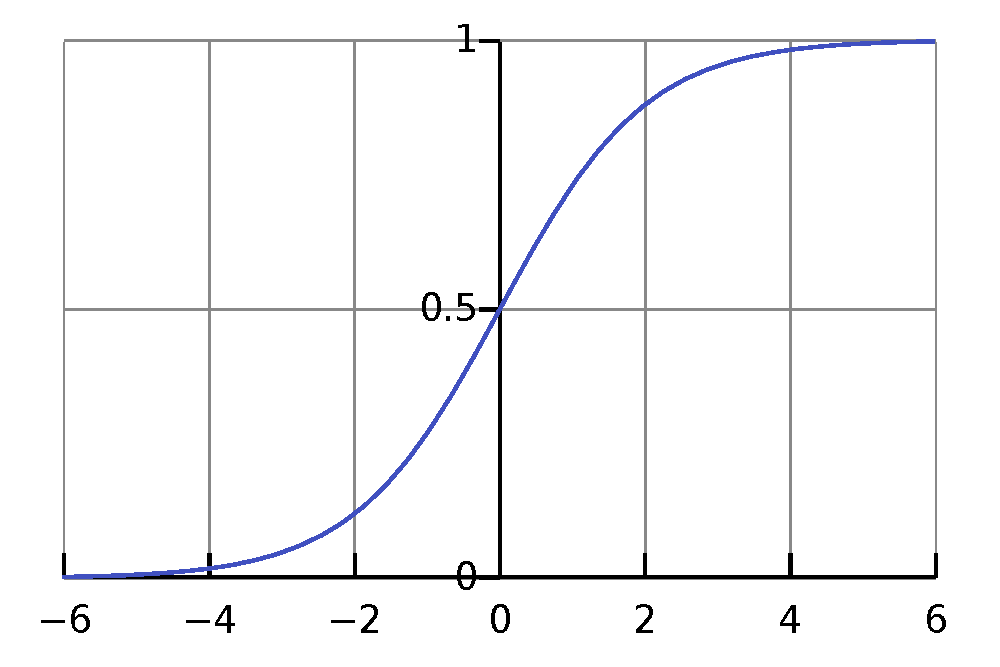
\includegraphics[scale=.5]{fig/Logistic-curve.pdf}
 \caption{The shape of the logistic curve. }
 \label{fig:logistic}
\end{figure}

\section{Backwards Phase: Propagation of Error Signal}
\label{sub:backwards_phase}
After the feedforward phase, the network is run in reserve in order to gather the weight adjustments. Unit $i$ sends the error signal:
\begin{equation}
  \delta_i = \eta_i (1 - \eta_i) (t_i - s_i)
\label{eq:bp_error}
\end{equation}
where $t_i$ is the target state. If $i$ is an output unit $t_i$ is the pre-set target pattern. Notice how the pre- and post-synaptic states of the unit are used to measure the error --- compare to how the output of the 2-layer perceptron was evaluated. This metric for calculating error is called cross-entropy error, other types (e.g., mean squared error) can also be used.

% \cite<using cross entropy, for rationale see:>{golik13}.
However, if $i$ is a hidden unit, its target is:

\begin{equation}
\label{eq:ff_targets}
  t_i = \sum_{j} \delta_j w_{ij} 
\end{equation}
meaning that the error signal $i$ emits is a function of the error signal emitted by the output units and the weights that connect them. 

\begin{enumerate}
 \item If the pre-synaptic activation of an output unit $i$ is $-6$ and its target $t_i$ is $1.0$, what error signal $d_i$ will it emit? (Use equations \ref{eq:ff_eta}, \ref{eq:logistic}, and \ref{eq:bp_error}.)
 
 \item What type of flow control statement is appropriate for calculating the $\sum$ is \autoref{eq:ff_targets}?
 
 \item What type of data is $i$ and what type of data is $s_i$?
 
 \item What are the main differences and similarities between the backwards and the feedforward phases of running a network?
 
 \item Why is the backwards phase required?
 
 \item How many types of target $t_i$ are there and why?
 
  \item Fill in the \texttt{Backprop()} function to run the network backwards. Use the inbuilt function \texttt{logit()} for the inverse of the logistic function.

 
 
 \end{enumerate}


\section{Weight Adjustments}
Once the network has been run forwards and backwards for an epoch, $\epsilon$, weight updates are calculated using:
% \begin{equation}
% \label{eq:ff_delta_weight}
% \Delta w_{ij} = \delta_j s_i
% \end{equation}
% for both the input-to-hidden and the hidden-to-output connection weights. The $\Delta w_{ij}$s are then applied to the current weights (at epoch $e$), to produce the new weights:
\begin{equation}
\label{eq:ff_adjusting_weights}
\Delta w_{ij}^{\epsilon} = - \mu \delta_j s_i + \nu \Delta w_{ij}^{\epsilon-1}
\end{equation}
taking into account the momentum, $\nu = 0.9$, and the learning rate, $\mu = 0.025$

% \cite{attohokine99, hertz91}.
% 


\bibliographystyle{apacite}
\bibliography{ref}
\end{document}
